%=================================================================
\section{Introduction}\label{sec-intro}
\par
The Kaggle Competition is aim to build a model that predicts the total ride duration of taxi trips in New York City.Kaggle provides us three files to help us complete this competition,which are train.csv,test.csv,submission.csv.
\par
The train.csv is aim to help us bulid a good model to make a prediction.There are some details about this file,seeing Figure \ref{five}
\begin{figure}[htbp]
	\centering
	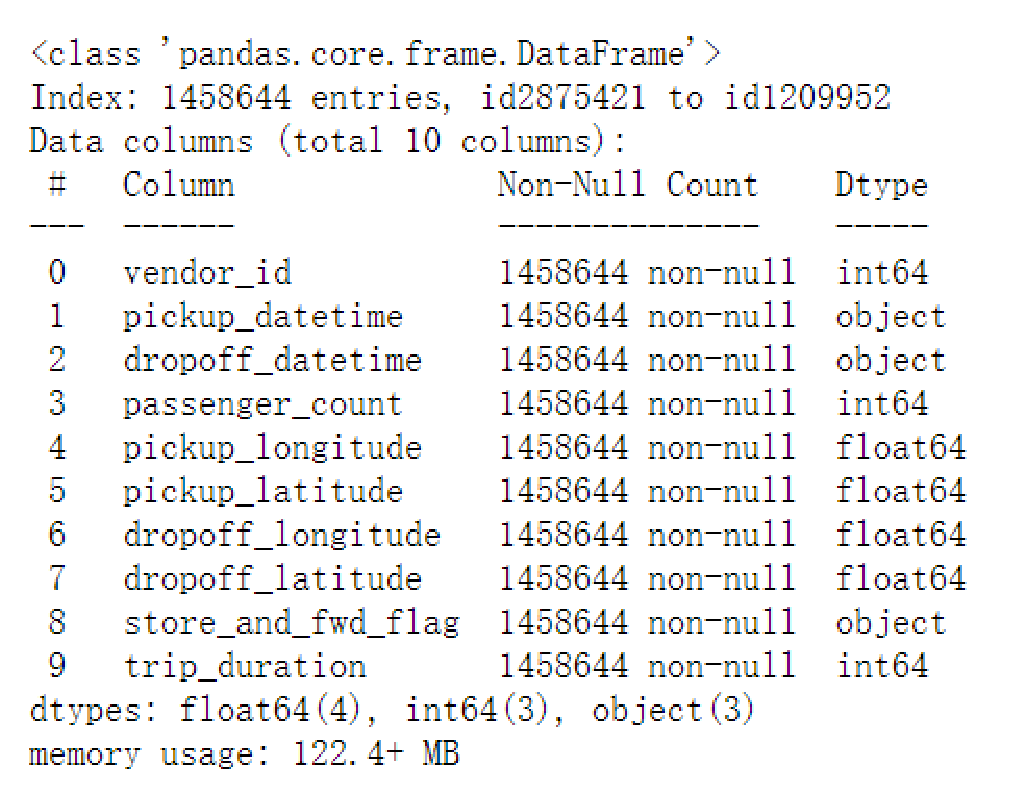
\includegraphics[scale=0.5]{figures/five.eps}
	\caption{Attributes of train data} \label{five}
\end{figure}
\par
The test.csv is aim to test the capability of the model you have trained.There are some details about this file,seeing Figure \ref{six}
\begin{figure}[htbp]
	\centering
	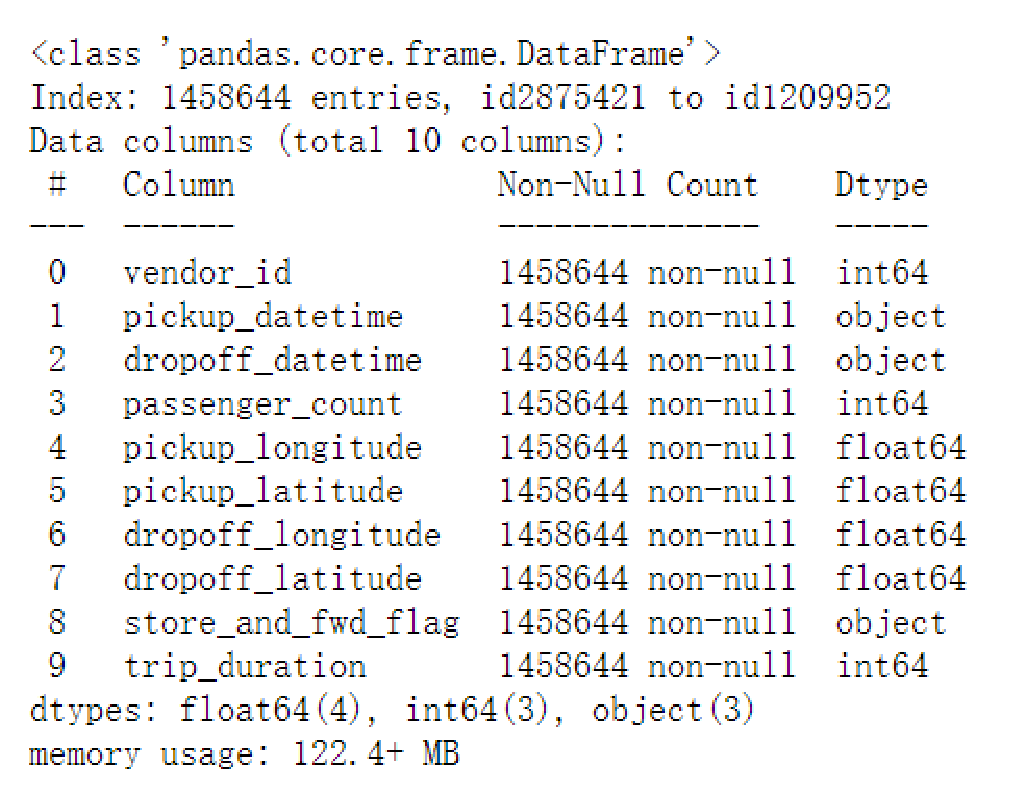
\includegraphics[scale=0.5]{figures/five.eps}
	\caption{Attributes of test data} \label{six}
\end{figure}
\newpage
The submission.csv is aim to provide format for submitting answers.
\par
In this competition,Our work is mainly divided into two steps,which are Data Processing and Model Selection.
\par
During data processing, we first do the data visualization,which will help us to find the stucture of the data and the law of data development.Throung this step, we can have a deeper sight into the data.
\par
After that,we can have better ideas for data processing.We will clean the data,since there are some items against common sense or missing attributes.Removing the oulters and Dealing with missing vlues is necessary.We also need to change type of some attributes,since some attributes have no quantitative relationship.Converting types of this attribute into string is a good choice.In some cases,we need to add some attributes to gain a better prediction.
\par
There are some good models to select,such as Ridge,Bagging,Boosting,RandomFor-
est,Lightgbm,Xgboost.In this process,the most crucial step is the choice of hyperparameters. There is no shortcut, only do constantly experimentations to find the best value during this process. 
%
%
%\todo{Narrow down to a topic; Dig a hole; Fill the hole}
%
%
%
%\gangli{``narrow in on topic'' reminds you 
%that readers and reviewers only know that this is a AI or HTM research paper (and maybe have read the title/abstract). 
%You need to help them figure out what topic and area of research paper this is. 
%You _don't_ need to wax poetic about the topic's importance.}
%
%\gangli{`dig a hole'' reminds you that 
%you need to convince the reader that there's a problem with the state of the world. 
%Prior work may exist but it's either missing something important or there's a missing opportunity. 
%The reader should be drooling for a bright future just out of reach.}
%
%\gangli{
%``fill the hole'' reminds you to show the reader 
%how and why the paper they're reading will fix these problems and deliver us into a better place. 
%You don't need a whirlwind summary of the technical details, 
%but you need readers convinced (and in a good mood) to keep reading.}
%
%
%
%\todo{The importance of the area}
%
%
%
%\todo{The problems faced by most current methods}
%
%
%\todo{What can be addressed by existing methods; Why those problems are challenges to existing methods?}
%\blindtext
%
%\todo{What provides the motivation of this work? What are the research issues? What is the rationale of this work? }
%\blindtext
%
%\todo{What we have done and what are the contributions.}
%\blindtext


%
%Test citation~\cite{BL12J01}. 
%\begin{JournalOnly}
%and~\citep{BJL11J01} or~\citet{BJL11J01}.
%\end{JournalOnly}
%
%This is for~\cref{tbl:overall-experiments}, 
%\todo[fancyline]{Testing.}
%and this is for~\cref{sec-conclusions}.
%\todo[noline]{A note with no line back to the text.}%
%\gangli{This is comment from Gang.}
%\qwu{Response from QW}
%
%Number:
%\num{123}.
%\numlist{10;30;50;70},
%\numrange{10}{30},
%\SIlist{10;30;45}{\metre},
%and
%\SI{10}{\percent}
%
%\missingfigure[figcolor=white]{Testing figcolor}
%
%
%\begin{ConferenceOnly}
%We have \SI{10}{\hertz},
%\si{\kilogram\metre\per\second},
%the range: \SIrange{10}{100}{\hertz}.
%$\nicefrac[]{1}{2}$.
%
%\missingfigure{Make a sketch of the structure of a trebuchet.}
%
%\end{ConferenceOnly}
%
%
%For~\cref{eq:test},
%as shown below:
%
%\begin{equation}\label{eq:test}
%a = b \times \sqrt{ab}
%\end{equation}
%
%\blindmathpaper

\section{Related Work} \label{sec-Related Work}
There are some popular models to trian the model.
\par
\textbf{Boosting} \quad Bagging puts a lot of small classifiers together, a random part of the data for each train, and then combines their final results (majority voting system).
\par
\textbf{Bagging} \quad Boosting is theoretically more advanced than Bagging, and it is also a classifier. But arrange them linearly. The next classifier adds a higher weight to the parts that were not well classified by the previous classifier, so that the next classifier can learn more "deeply" in this part.
\par
\textbf{Random Forest} \quad Random forests or random decision forests are an ensemble learning method for classification, regression and other tasks that operates by constructing a multitude of decision trees at training time and outputting the class that is the mode of the classes (classification) or mean/average prediction (regression) of the individual trees. Random decision forests correct for decision trees' habit of overfitting to their training set.Random forests generally outperform decision trees, but their accuracy is lower than gradient boosted trees. However, data characteristics can affect their performance.

%\blindtext
%
%\gliMarker  %TODO: GLi Here

\section{Method} \label{sec-method}

\subsection{Data Processing}
There are two main steps.
\par
\textbf{Data Vasulization} \quad Frist,we analyze the correlation of attributes.We use Spearman Correlation instead of Person corrlation.
The results can be seen in Figure \ref{two}.From the figure, we can see that latitude has the greatest impact on duration, and we need to emphasize on this attribute greatly.
\par
\begin{figure}[htbp]
	\centering
	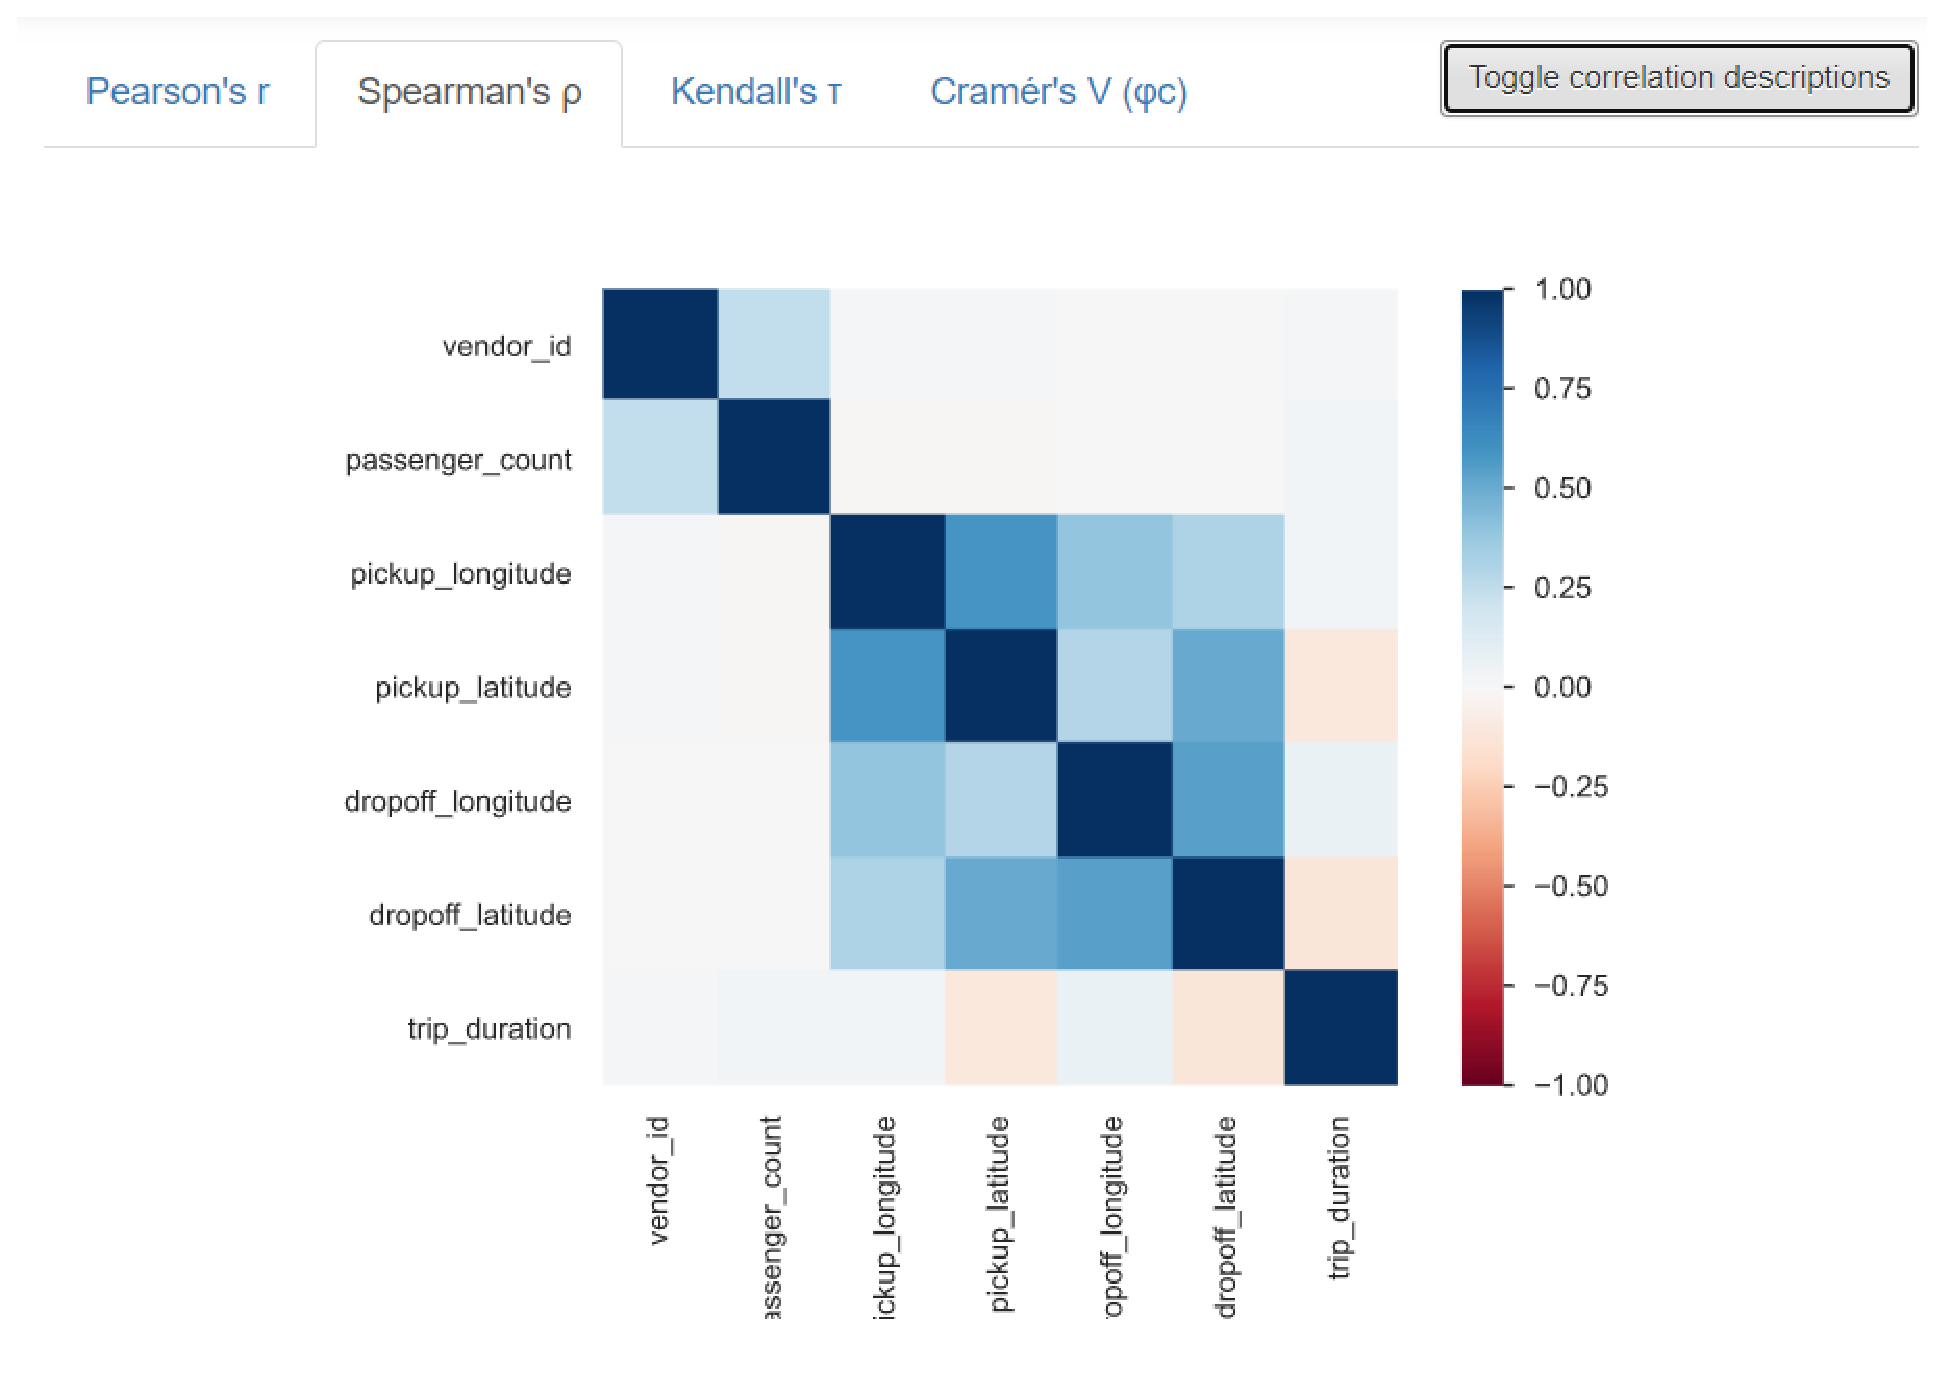
\includegraphics[scale=0.4]{figures/two.eps}
	\caption{Correlation of Attributes} \label{two}
\end{figure}
\par For the attribute named vendor\_id,it's a code indicating the provider associated with the trip record.We can see it's distribution in Figure\ref{three}.It's worth noting that it's type is int.We need to convert it into string for one-hot encoding.
\begin{figure}[htbp]
	\centering
	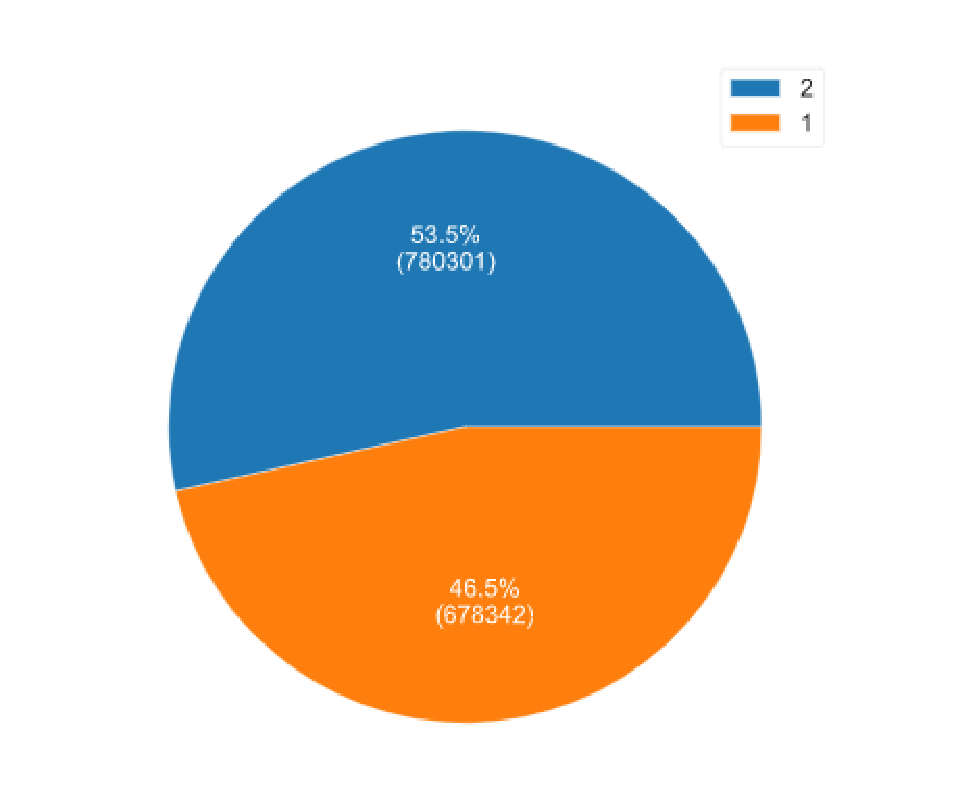
\includegraphics[scale=0.4]{figures/three.eps}
	\caption{Proportion of different values of vendor\_id} \label{three}
\end{figure} 
\par For the attibute named store\_and\_fwd\_flag,it's a flag indicates whether the trip record was held in vehicle memory before sending to the vendor, because the vehicle did not have a connection to the server - Y=store and forward; N=not a store and forward trip.Proportion of different values of this attribute can be seen in Figure \ref{four}
\begin{figure}[htbp]
	\centering
	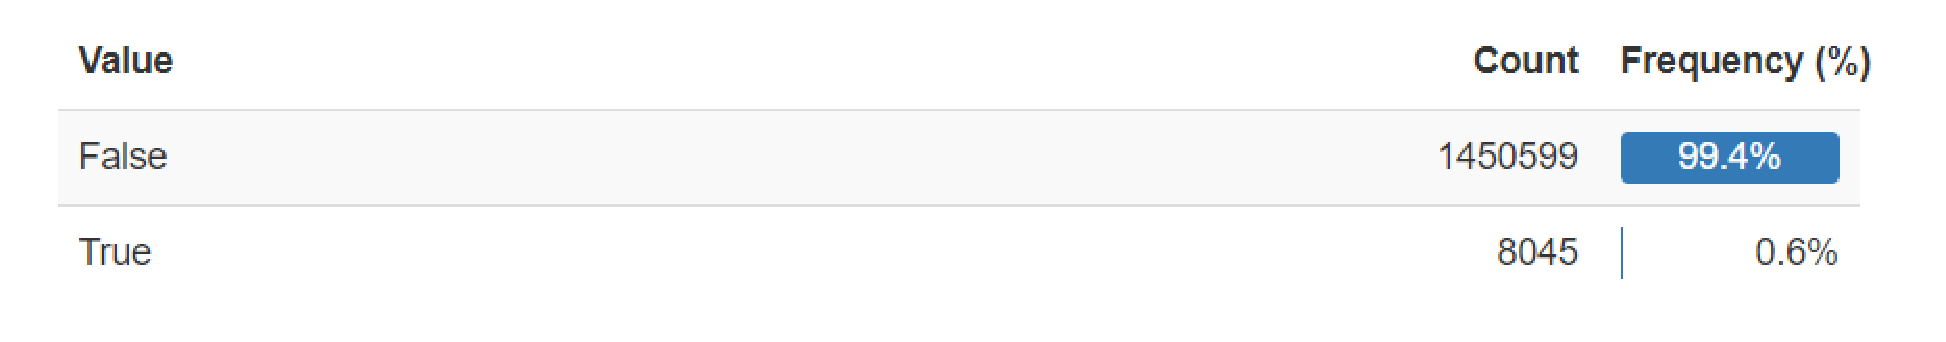
\includegraphics[scale=0.4]{figures/four.eps}
	\caption{Proportion of different values of store\_and\_fwd\_flag} \label{four}
\end{figure} 
\par For the attibute named passenger\_count,it means the number of passengers in the vehicle (driver entered value).From figure \ref{seven},we can find there is some data whose passenger\_count is more than 6.Howerver,such a large-capacity taxi does not exist.Therefore,we need to remove these items.
\begin{figure}[htbp]
	\centering
	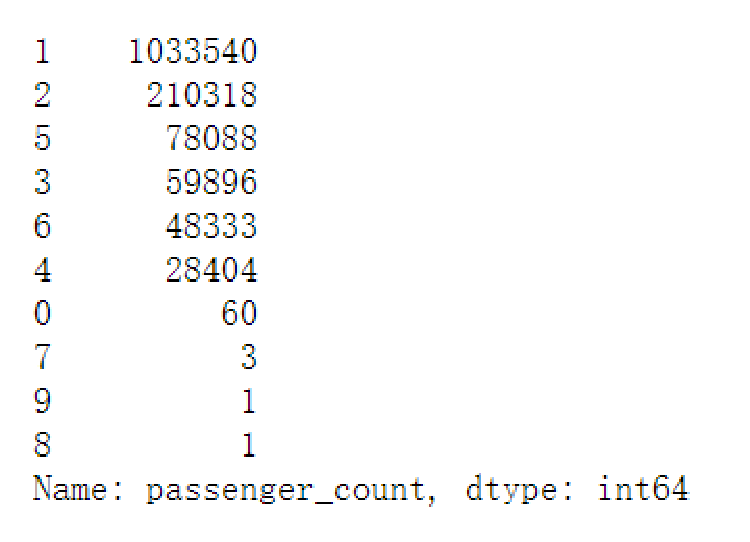
\includegraphics[scale=0.4]{figures/seven.eps}
	\caption{Number of trips for different passenger\_count} \label{seven}
\end{figure}

\par For the attibute named dropoff\_datetime,which doesn't exist in test,it means it's useless for prediction based on test.csv.There,we need to remove this attribute.

\par For the attibute named pickup\_datetime,we first divide it into  month, day, hour. From Figure\ref{nine},Figure\ref{12},we can see month,day and hour truely affect trip duration.However,if we direclty use one-hot encoding on the attributes(day and hour), it will cause disaster of dimensionarity.Therefore,we need to divide them into different categories.Moreover,We can deduce the day of the week from the date.From Figure\ref{13},it's useful to add this attribute.  

\begin{figure}[htbp]
	\centering
	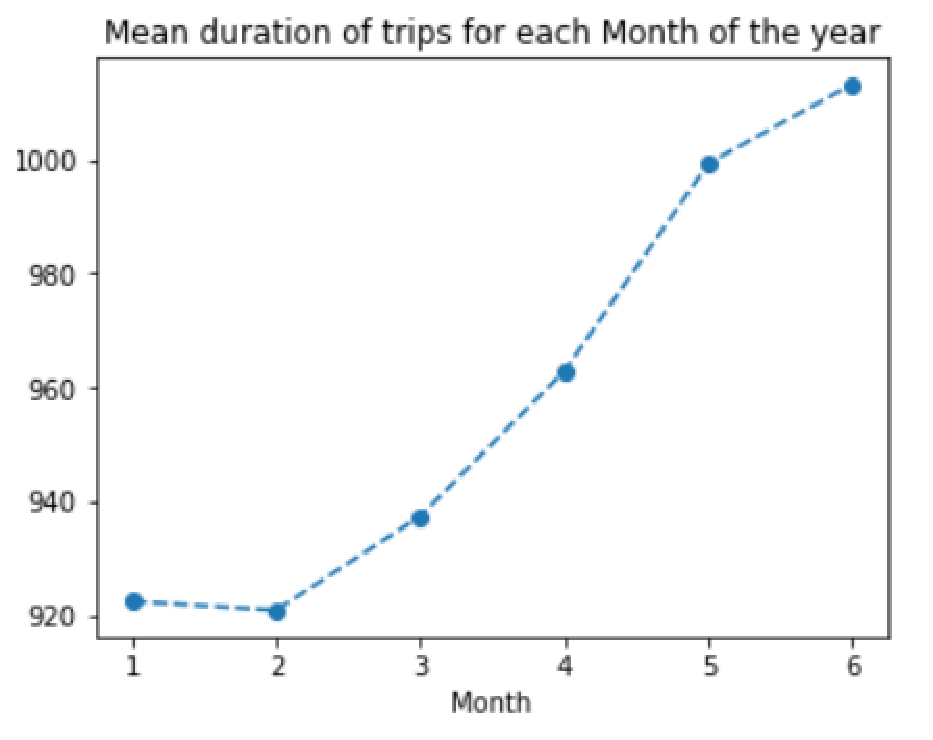
\includegraphics[scale=0.4]{figures/nine.eps}
	\caption{Mean trip duration of month } \label{nine}
\end{figure}

\begin{figure}[htbp]
	\centering
	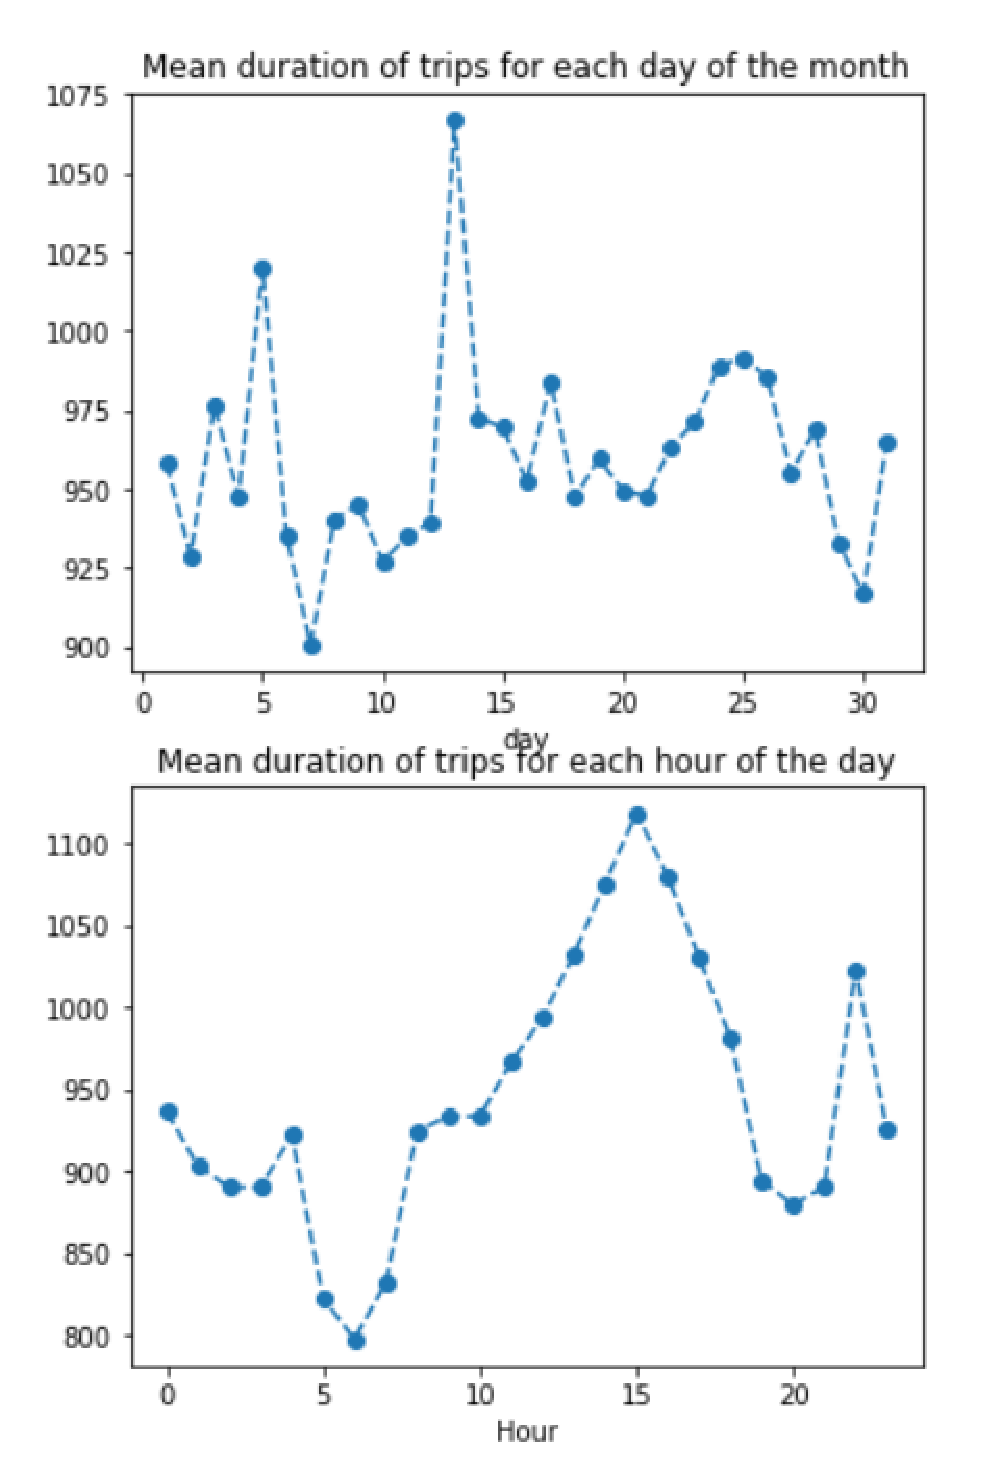
\includegraphics[scale=0.4]{figures/12.eps}
	\caption{Mean trip duration of day and hour } \label{12}
\end{figure}

\begin{figure}[htbp]
	\centering
	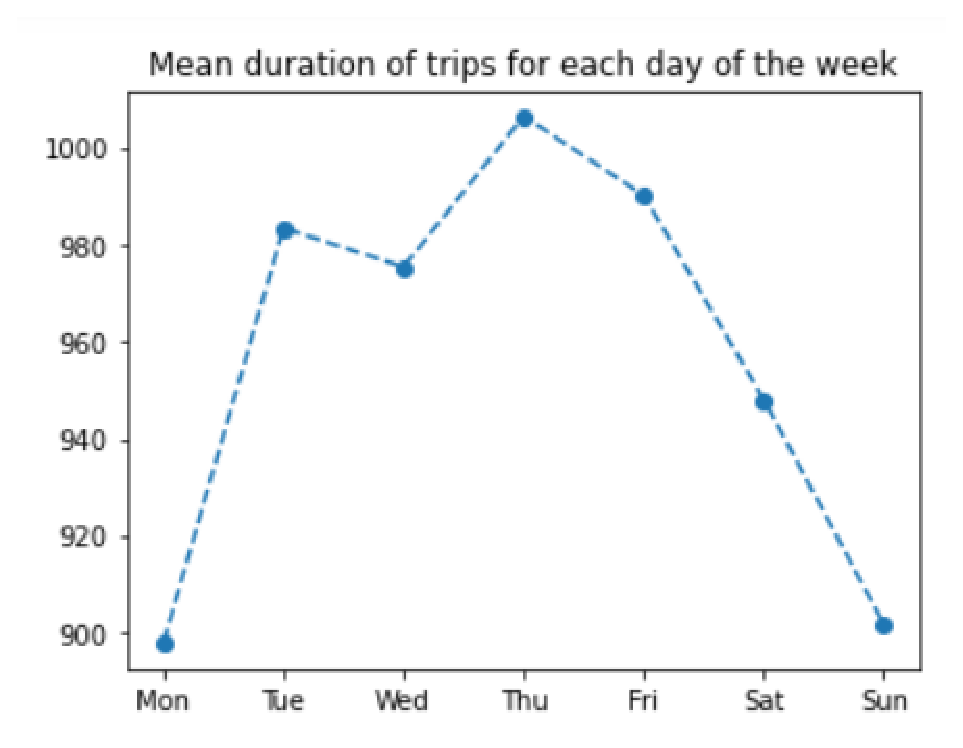
\includegraphics[scale=0.4]{figures/13.eps}
	\caption{Mean trip duration of weekday } \label{13}
\end{figure}

\par As we all know, time is equal to distance divided by speed.Therefore,I introduced the distance between Euclidean and Manhattan through latitude and longitude in order to predict better.
\par On the other hand,the speed of taxis is different in different areas, such as urban areas and suburbs.So I divided the city into five clusters in term of longitude and latitude.You can see the result in Figure\ref{15}.
\par I also introduced the azimuth angle through the latitude and longitude, because it will affect the speed to a certain extent.
\begin{figure}[htbp]
	\centering
	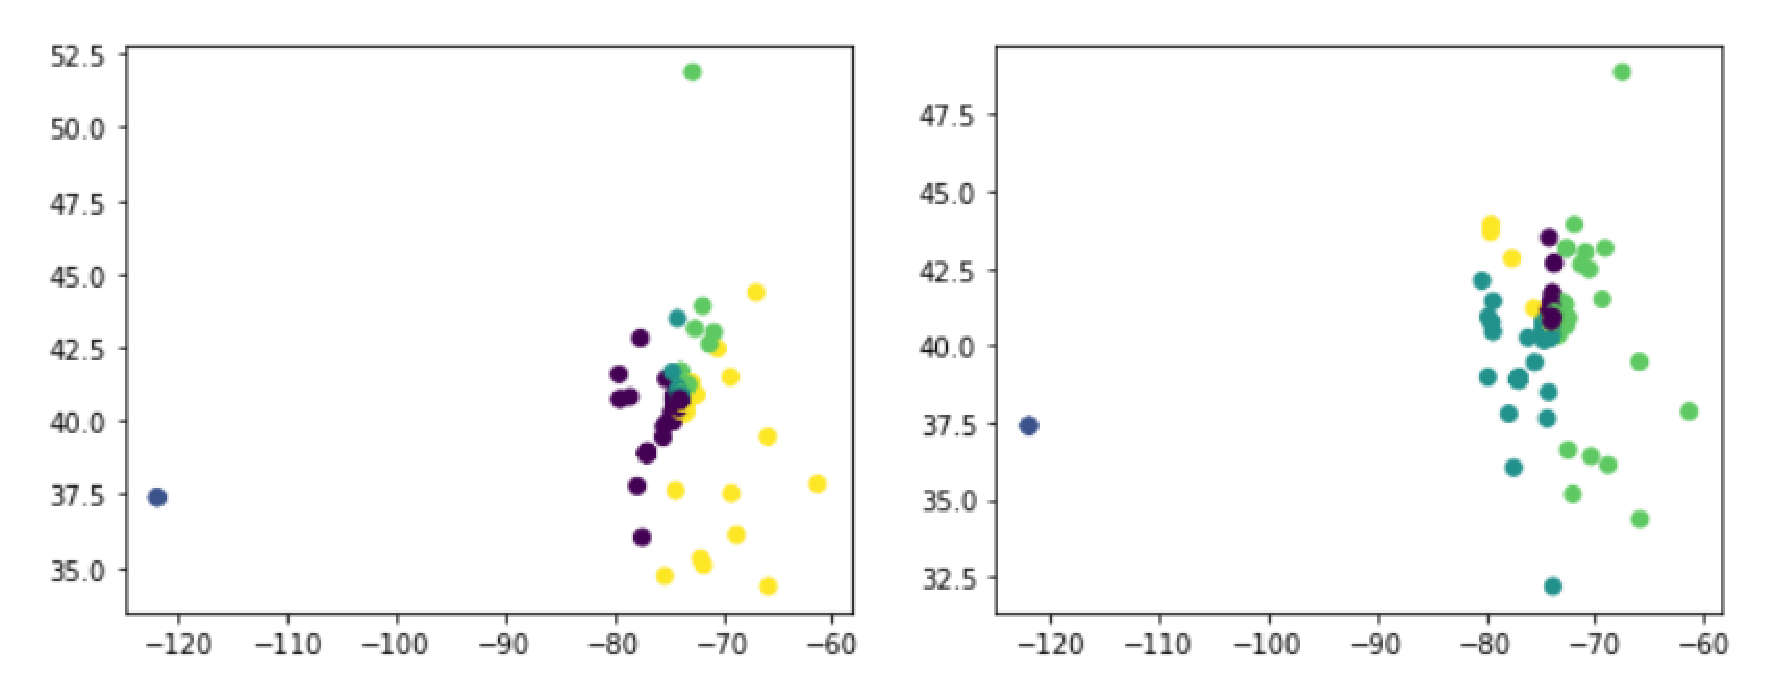
\includegraphics[scale=0.4]{figures/15.eps}
	\caption{Clusters of pick\_up and drop\_off locations } \label{15}
\end{figure}
\par I marked the pick-up and drop-off location by latitude and longitude,in Figure \ref{16}.From Google,we know New York City longitude vary from -74.03 to -73.75,and latitude vary from 40.63 to 40.85.In term of this, we remove some items.
\begin{figure}[htbp]
	\centering
	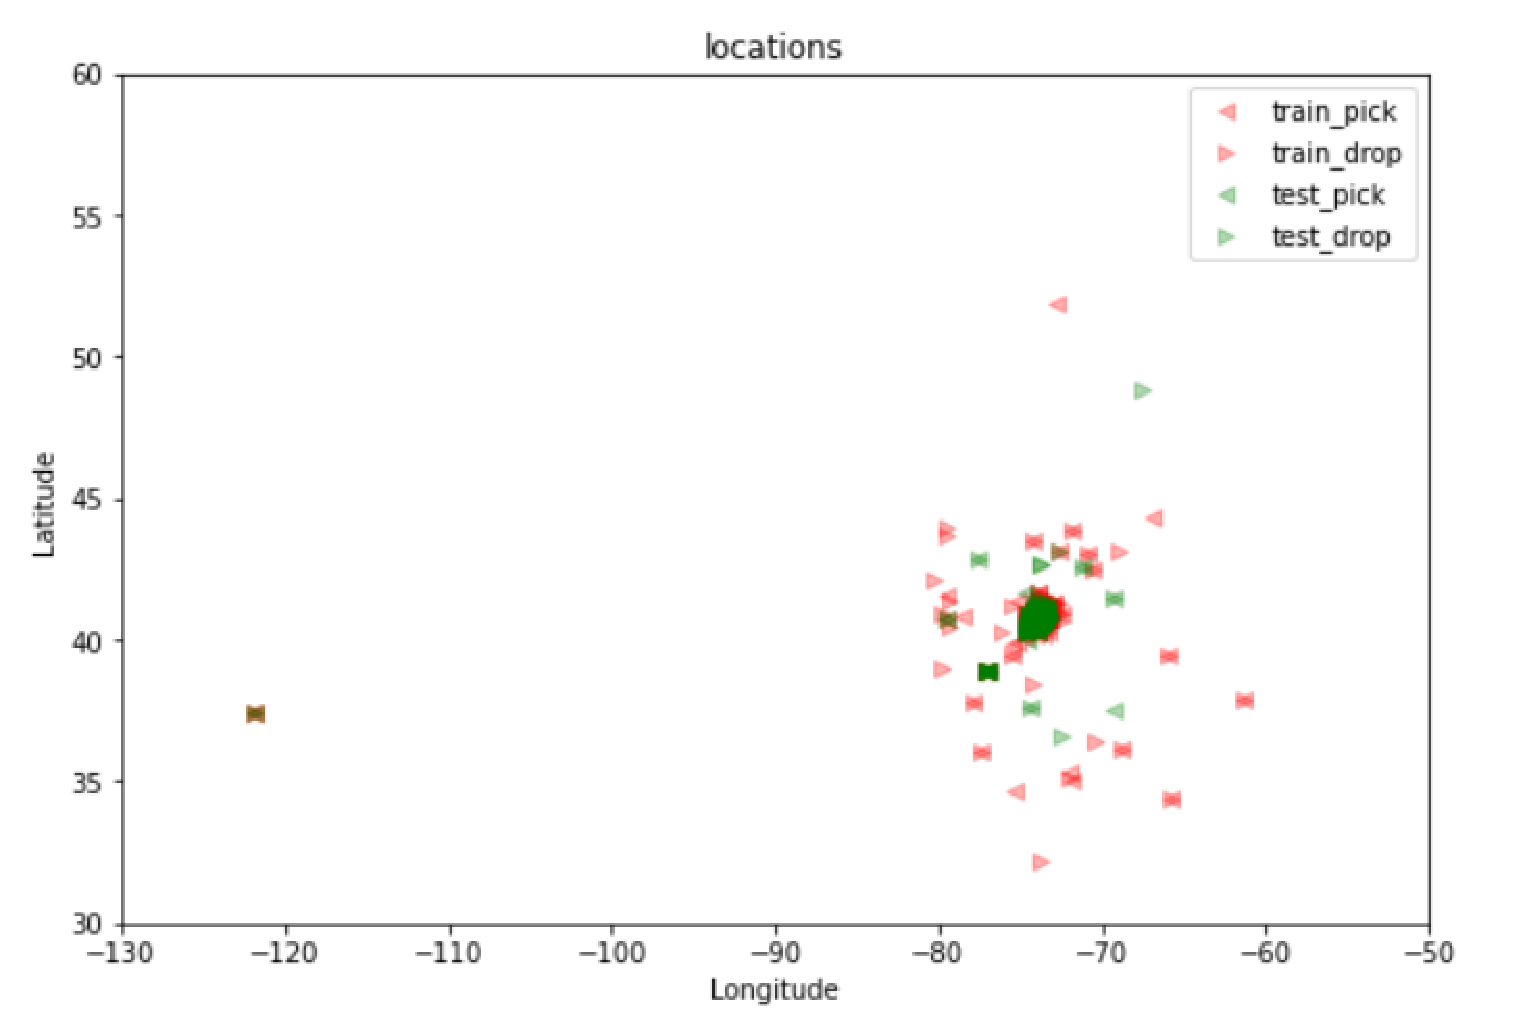
\includegraphics[scale=0.4]{figures/16.eps}
	\caption{Clusters of pick\_up and drop\_off locations } \label{16}
\end{figure}

\par For the attibute named trip\_duration,it's distribution can be seen in Figure\ref{17}.We can use power conversion to make it more like Gaussian distribution.
This can improve our prediction accuracy.The distribution can be seen in Figure\ref{18} after power conversion.
\begin{figure}[htbp]
	\centering
	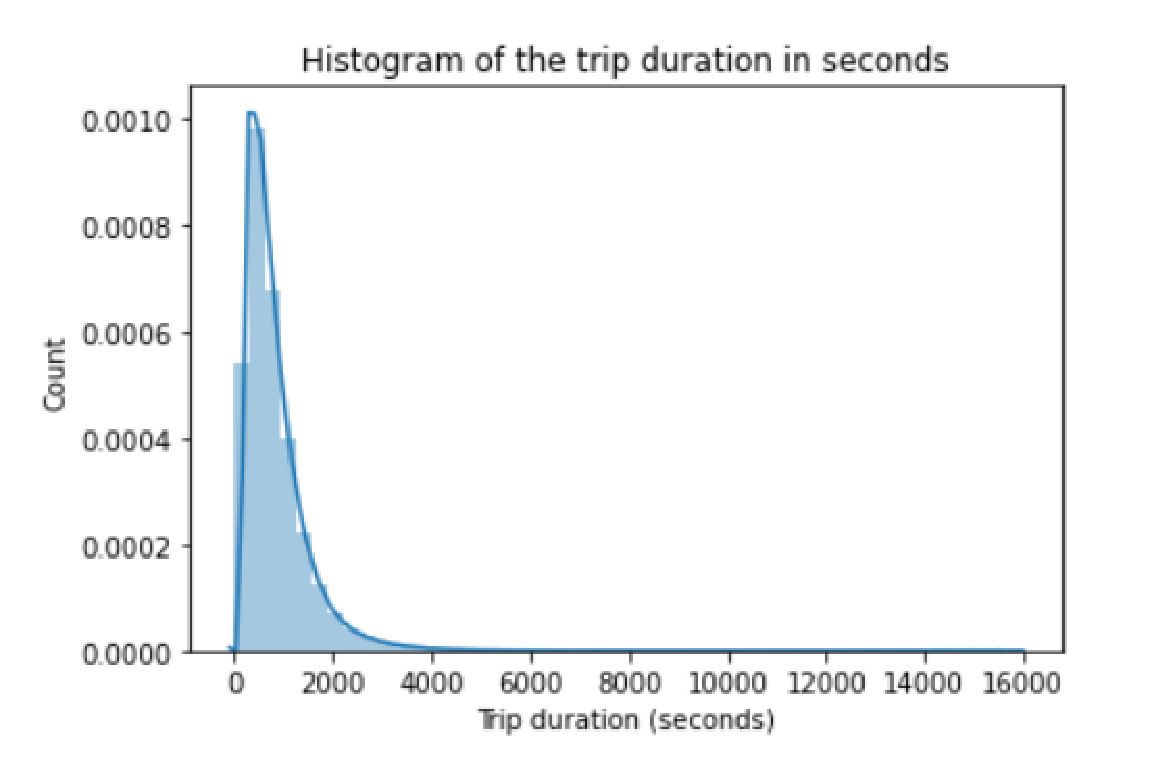
\includegraphics[scale=0.4]{figures/17.eps}
	\caption{Distribution of trip\_duration } \label{17}
\end{figure}

\begin{figure}[htbp]
	\centering
	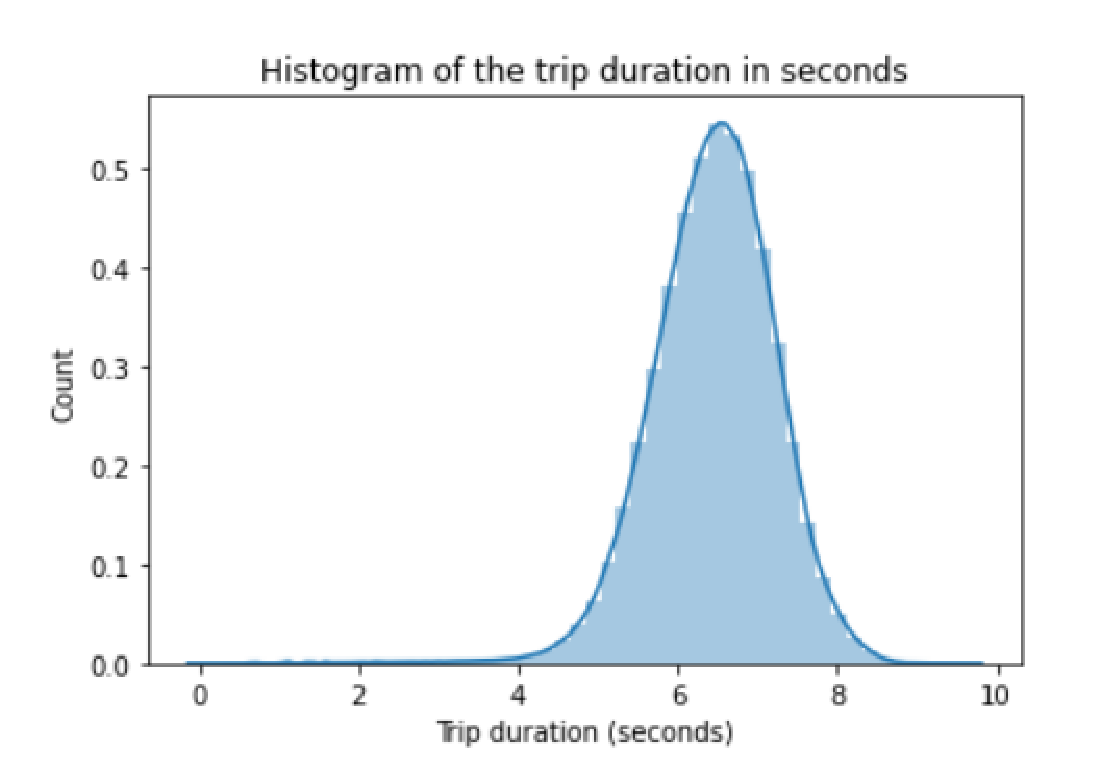
\includegraphics[scale=0.4]{figures/18.eps}
	\caption{Distribution of trip\_duration after power conversion } \label{18}
\end{figure}

\subsection{Model selection}
There are some popular Models,such as Ridge,Bagging, Boosting,RandomForest,Lightgbm,Xgboost.In our Competition, Lightgbm and Xgboost perform best.It's result can be seen in Figure\ref{24},Figure\ref{20}.
\begin{figure}[htbp]
	\centering
	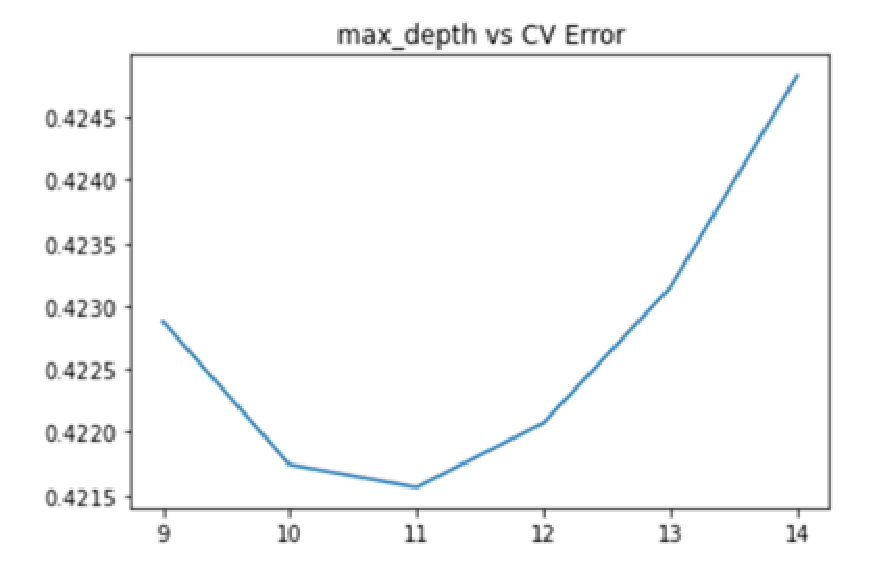
\includegraphics[scale=0.4]{figures/20.eps}
	\caption{ Xgboost } \label{20}
\end{figure}
\begin{figure}[htbp]
	\centering
	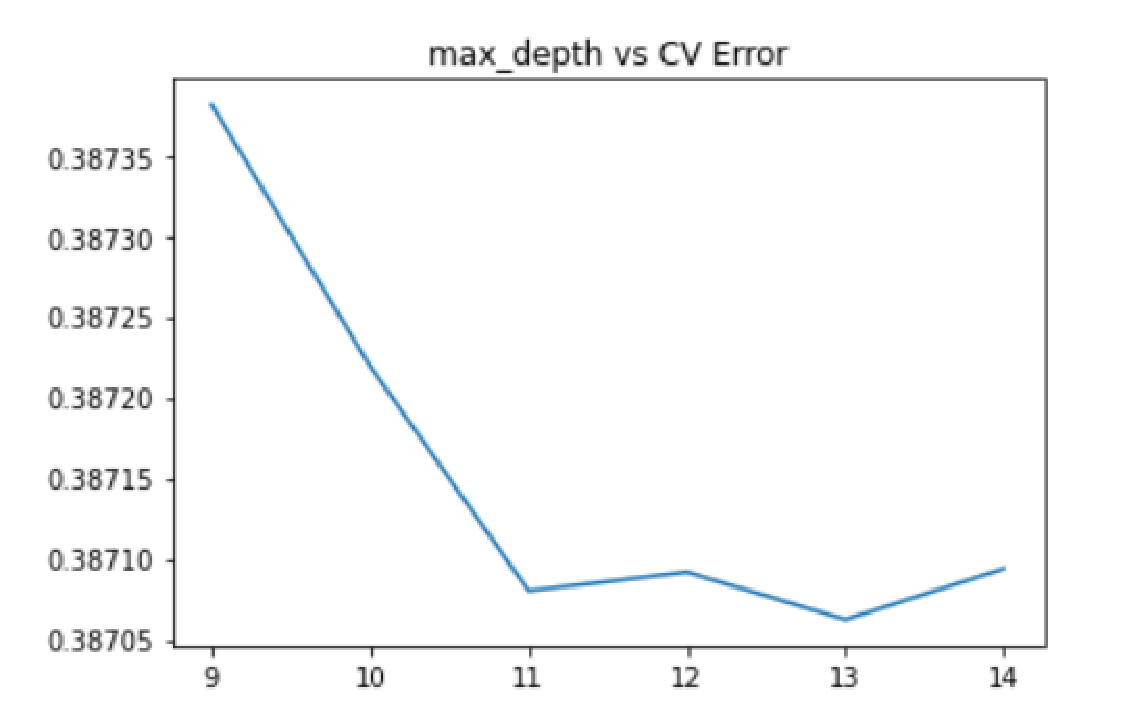
\includegraphics[scale=0.4]{figures/24.eps}
	\caption{Lightgbm } \label{24}
\end{figure}
%\blindtext
%\blindlist{itemize}[3]
%\blinditemize
%\blindenumerate
%
%\blindmathtrue
%\blindmathfalse
%\blinddescription
%
%\qwuMarker %TODO: QWu Here

\section{Experiment and Analysis} \label{sec-experiment}


%\begin{table}  \centering
%  \caption{Precision Comparison on Event Detection Methods}
%  \label{tbl:overall-experiments}
%  \begin{tabular}{cccc}
%\toprule
%    % after \\: \hline or \cline{col1-col2} \cline{col3-col4} ...
%    & OR Event Detection & AC Event Detection & TC Event Detection \\
%\midrule
%    precision & 0.83 & 0.69 & 0.46 \\
%    recall & 0.68 & 0.48 & 0.36 \\
%    F-score & 0.747 & 0.57 & 0.4 \\
%\bottomrule
%\end{tabular}
%\end{table}


\section{Conclusions} \label{sec-conclusions}

\blindtext

\section*{Acknowledgement}

\lipsum[1]


The authors would like to thank \ldots

